\documentclass[fontsize=12pt]{scrartcl}

%Settings-Datei einbinden
% !TEX root = Bachelorarbeit_Paul_Zilewitsch.tex
\usepackage{comment}
\usepackage{amsmath}
\usepackage{amssymb}

% deutsche Silbentrennung
\usepackage[ngerman]{babel}

% deutsche Umlauten
\usepackage[T1]{fontenc}
\usepackage{inconsolata}
\usepackage[utf8]{inputenc}

%Anführungszeichen
\usepackage[autostyle=true,german=quotes]{csquotes}

%Zeilenabstand 1,5 
\usepackage[onehalfspacing]{setspace}

%Times New Roman
\usepackage{mathptmx}
\setkomafont{disposition}{\rmfamily}

%Arrays, Tabellen und Listen
\usepackage{array}
\usepackage{tabto}
\usepackage{longtable}
\usepackage{supertabular}

%Seitenzahlen
\usepackage{scrpage2}
\cfoot[]{}
\ofoot[\pagemark]{\pagemark}
\pagestyle{scrheadings}

%Inhaltsverzeichnis
\usepackage{tocloft}
\usepackage{titletoc}
\cftsetindents{section}{0.0in}{0.5in}
\cftsetindents{subsection}{0.0in}{0.5in}
\cftsetindents{subsubsection}{0.0in}{0.5in}
\cftsetindents{paragraph}{0.0in}{0.5in}
\renewcommand{\cftsecleader}{\cftdotfill{\cftdotsep}}
\renewcommand\cftsecfont{\mdseries}
\renewcommand\cftsecpagefont{\mdseries}
\renewcaptionname{ngerman}{\contentsname}{} %kein Titel für Inhaltsv. 
%\usepackage{hyperref} %für links im inhaltsverzeichnis

%Abkürzungsverzeichnis
\usepackage{enumitem} 

%Abbildungsverzeichnis
\renewcaptionname{ngerman}{\listfigurename}{}

\titlecontents{figure}
  [0em]
  {}
  {\figurename\enspace\thecontentslabel:\enspace}
  {}
  {\titlerule*[1pc]{.}\contentspage}
  
  %Tabellenverzeichnis
\renewcaptionname{ngerman}{\listtablename}{}

\titlecontents{table}
  [0em]
  {}
  {\tablename\enspace\thecontentslabel:\enspace}
  {}
  {\titlerule*[1pc]{.}\contentspage}

%Seitenränder
\usepackage{geometry}
\geometry{a4paper, top=21mm, left=30mm, right=20mm, bottom=20mm,
headsep=10mm, footskip=10mm}

%C# Code-Anzeige
\usepackage{color}
\definecolor{bluekeywords}{rgb}{0.13,0.13,1}
\definecolor{greencomments}{rgb}{0,0.5,0}
\definecolor{redstrings}{rgb}{0.9,0,0}

\usepackage{listings}
\lstset{language=[Sharp]C,
  showspaces=false,
  showtabs=false,
  breaklines=true,
  showstringspaces=false,
  breakatwhitespace=true,
  escapeinside={(*@}{@*)},
  commentstyle=\color{greencomments},
  keywordstyle=\color{bluekeywords},
  stringstyle=\color{redstrings},
  basicstyle=\ttfamily
}

%Überschriften Definition
\usepackage{titlesec}

\titleformat{\section}
  {\normalfont\fontsize{16}{17}\rmfamily\bfseries}
  {\thesection}
  {2em}
  {}

\titleformat{\subsection}
  {\normalfont\fontsize{14}{17}\rmfamily\bfseries}
  {\thesubsection}
  {1.5em}
  {}
  
  \titleformat{\subsubsection}
  {\normalfont\fontsize{14}{17}\rmfamily\mdseries}
  {\thesubsubsection}
  {0.75em}
  {}
\titlespacing{\section}{0pt}{*6}{*5} %{Einzug} {abstand nach oben}{abstand nach unten}
\titlespacing{\subsection}{0pt}{*5}{*3}
\titlespacing{\susubbsection}{0pt}{*4}{*2}

%Fußnoten
\usepackage[multiple, hang]{footmisc} % Komma zwischen mehreren Fußnoten
\setlength{\footnotemargin}{1em}
%\usepackage[justification=RaggedRight, singlelinecheck=false]{caption}
%\usepackage{caption}
%\captionsetup{%
%  textfont=footnotesize,
%  labelfont=footnotesize,
%  font=singlespacing,
%}


%Bilder
\usepackage{graphicx}


%Farben und Zeichnungen
\usepackage{pict2e}  
\usepackage{color}
\usepackage{ amssymb }
\definecolor{gray}{RGB}{150, 150, 150}


%Literaturverzeichnis
%\bibliographystyle{apalike} 
\bibliographystyle{unsrtnat} 
\usepackage[numbers,round,sort]{natbib}
\addto\captionsngerman{\renewcommand{\refname}{Literaturverzeichnis}}






\begin{document}

%-------------------------------------------------------------------------------------------------------
%					Titelseite
%-------------------------------------------------------------------------------------------------------
\thispagestyle{empty}
\large
	%noindent = kein absatzeinzug
	\noindent Berufsakademie Sachsen \hfill KMS Computer GmbH\\
	Staatliche Studienakademie Dresden \\
	Studiengang Informationstechnik
	%\includegraphics[width=0.5\textwidth]{ba-logo.png}
\begin{center}	
	\vspace*{4cm}
	\textbf{Konzipierung und prototypische Entwicklung einer E-mail Integration auf Basis der Microsoft Exchange Web Services im Service Desk der CAFM Software GEBman 10}\\
	\vspace*{2cm}
		Bachelorarbeit\\ zur Erlangung des Abschlusses\\ Bachelor of Engineering\\ im Studiengang 						Informationstechnik\\
	\vspace*{2cm}
	eingereicht von:\\Zilewitsch, Paul
	\vspace*{3cm}
\end{center}
	1. Gutachter: Dr. rer. nat., Dipl.-Chem. Hansi Schilling\\
	2. Gutachter: B.Sc. Sebastian Schulze 
	\\\\
	\begin{tabular}{@{}ll}
		Tag der Themenübergabe:&22.04.2016\\
		Tag der Einreichung:&18.07.2016
	\end{tabular}
\pagebreak


%-------------------------------------------------------------------------------------------------------
%					Auftragsblatt lose hineinlegen, wird aber mitgezählt
%-------------------------------------------------------------------------------------------------------



%-------------------------------------------------------------------------------------------------------
%					Autorenreferat
%-------------------------------------------------------------------------------------------------------
\noindent
\Large\bfseries
Autorenreferat
\normalsize\mdseries
\thispagestyle{empty}
\newline\newline
\noindent
ZILEWITSCH, Paul: Konzipierung und prototypische Entwicklung einer E-mail Integration auf Basis der Microsoft Exchange Web Services im Service Desk der CAFM Software GEBman 10,  Berufsakademie Sachsen, Staatliche Studienakademie Dresden, Studiengang Informationstechnik, Bachelorarbeit, 2016.\\ 
XXX Seiten, XXX Literaturquellen , XXX Anlagen. 
\newpage

%-------------------------------------------------------------------------------------------------------
%					Inhaltsverzeichnis
%-------------------------------------------------------------------------------------------------------
\addsec{Inhaltsverzeichnis} %vergebe keine Kapitelnummer\\
\vspace*{-1cm}
\pagenumbering{Roman}
\setcounter{page}{4}
\tableofcontents 
\newpage

%-------------------------------------------------------------------------------------------------------
%					Abbildungsverzeichnis
%-------------------------------------------------------------------------------------------------------
\addsec{Abbildungsverzeichnis} %vergebe keine Kapitelnummer
\vspace*{-1cm}
\listoffigures
\newpage

%-------------------------------------------------------------------------------------------------------
%					Abkürzungsverzeichnis
%------------------------------------------------------------------------------------------------------
\addsec{Abkürzungsverzeichnis} %vergebe keine Kapitelnummer
\begin{enumerate}
\item[1] CAFM \tabto{3cm} Computer-Aided Facility Management
\item[2] ITIL \tabto{3cm} Information Technology Infrastructure Libary
\item[3] HTTP \tabto{3cm} Hypertext Transfer Protocol
\item[4] HTTPS \tabto{3cm} Hypertext Transfer Protocol Secure
\item[5] API \tabto{3cm} Application Programming Interface
\item[6] REST API \tabto{3cm} Representational State Transfer Application Programming Interface
\item[7] SOAP \tabto{3cm} Simple Object Access Protocol
\item[8] XML \tabto{3cm} Extensible Markup Language
\item[9] SPoC \tabto{3cm} Single Point of Contact

\end{enumerate}
\newpage

%-------------------------------------------------------------------------------------------------------
%					Tabellenverzeichnis
%-------------------------------------------------------------------------------------------------------
\addsec{Tabellenverzeichnis} %vergebe keine Kapitelnummer
%\listoftables
\newpage

%-------------------------------------------------------------------------------------------------------
%					1	Einleitung
%-------------------------------------------------------------------------------------------------------


\pagenumbering{arabic}     
\setcounter{page}{1}
% !TEX root = Bachelorarbeit_Paul_Zilewitsch.tex
\section{Einleitung}

%http://webuser.hs-furtwangen.de/~kaspar/seminar0405/Service_Desk.pdf

\subsection{Die Software GEBman 10 von der KMS Computer GmbH}
\noindent
Die IT ist ein ständiger Begleiter im Arbeitsalltag eines jeden Unternehmens. Sie erleichtert nicht nur die Arbeit mit großen Datenmengen, sondern unterstützt auch wichtige Geschäftsprozesse in -und außerhalb des Unternehmens. Um einen möglichst effizienten Einsatz der IT zu ermöglichen, halten sich viele Unternehmen an bestimmte Best Practice Frameworks. Diese Leitfäden beinhalten unter anderem den Einsatz der IT im Bereich Kundenservice. Dabei übernimmt ein sogenannter Service Desk eine wichtige Funktion. Diese zentrale Anlaufstelle dient als Kommunikationsschnittstelle zwischen dem Kunden und der IT-Organisation. Viele Unternehmen setzen auf eine externe Service Desk-Softwarelösung, die dem Support eine bessere Kommunikation mit dem Kunden und ein effizienteres Abarbeiten von Vorfällen ermöglicht.\\

\noindent
Die KMS Computer GmbH bietet ebenfalls eine Lösung eines Service Desk an, die jedoch auf den Bereich Facility Management spezialisiert ist. Das Unternehmen wurde 1990 gegründet und konzentriert sich heute vorrangig auf den Vertrieb von entwickelter Software im Bereich Computer-Aided Facility Management (CAFM). Computer-Aided bedeutet so viel wie \enquote{computergestützt}. Den Begriff Facility Management beschreibt der Spezialist für Gebäude- und Immobilienwirtschaft Nävy präzise \enquote{als strategische Management-Disziplin, die die Analyse, Dokumentation und Optimierung aller kostenrelevanten Vorgänge rund um Gebäude und ihre Anlagen und Einrichtungen (Facilities) unter besonderer Berücksichtigung von Arbeitsplatz und Umfeld der Nutzer umfaßt.}\footnote{\citeauthor{Naevy} (\citeyear{Naevy}), S. VII}\\

\noindent
Seit 2011 entwickelt und vertreibt die KMS Computer GmbH die webbasierte Software GEBman 10. Es handelt sich bei GEBman 10 um eine CAFM-Software für Kommunen, Industrie und Gebäudeverwalter. Übersichten geografischer Informationen oder die Analyse von Sachdaten können individuell auf die Kunden abgestimmt werden. Außerdem ist es ein Werkzeug zur Verwaltung und ein Arbeitsmittel zur Unternehmensführung oder der finanziellen Planung. Die Anwendung kann als Desktop-Installation, als interne Weblösung oder als Cloud-Lösung betrieben werden. Aber auch mobile Lösungen einzelner Module sind bereits in Verwendung und werden stetig weiterentwickelt. Es wird schon jetzt deutlich, dass GEBman 10 mannigfaltig ist und mit über 40 Modulen auch in vielen Branchen zum Einsatz kommt. Gerade in sehr speziellen Bereichen, wie beispielsweise Außenbeleuchtung oder Baumverwaltung, kann es zu den unterschiedlichsten und ungewöhnlichsten Problemen kommen. Eine Grundvoraussetzung  für die effiziente Lösung von Problemen, ist das Festhalten der genauen Vorkommnisse. Hierbei kann das Modul Service Desk in GEBman 10 durchaus hilfreich sein und alle erforderlichen Prozesse zur Problemlösung unterstützen.



\subsection{Das Modul Service Desk}
\noindent
Der Service Desk in GEBman 10 ist stark an die anderen Module gebunden und auf den Bereich Facility Management ausgelegt. Im Modul Service Desk ist es möglich, Meldungen für verschiedenste Objektarten aufzugeben. Ist beispielsweise eine Außenbeleuchtung eines Gebäudes ausgefallen, kann ein Benutzer eine Störmeldung bezüglich der Außenbeleuchtung aufgeben. Dabei wählt er das entsprechende Gebäude aus und trägt die genaue Problemstellung in die Meldung ein. So hat ein Techniker zum Beispiel die Möglichkeit, in die Störmeldung Einsicht zu nehmen und die defekte Außenbeleuchtung zu reparieren. Oder aber er fragt nach den genauen Ursachen und antwortet somit auf die Störmeldung. Probleme und Vorfälle können durch den Service Desk genau spezifiziert und archiviert werden. Dadurch ist eine effizientere Lösung des Problems bei einem erneuten Auftreten möglich.\\


\subsection{Motivation der Arbeit}
\noindent
Die KMS Computer GmbH nutzt derzeit eine externe Service Desk-Software, um sämtliche Vorfälle in der Support-Abteilung zu bearbeiten und zu protokollieren. Ziel der Bachelorarbeit ist es, das Service Desk Modul in GEBman10 so anzupassen, dass auf eine externe Service Desk-Lösung verzichtet und das hauseigene Produkt eingesetzt werden kann. Dadurch könnten nicht nur die Kosten für die Lizenzierung der externen Lösung eingespart, sondern ein effektiveres Arbeiten mit der eigenen Servie Desk-Lösung ermöglicht werden. Hierfür muss das Modul Service Desk um eine E-Mail-Integration erweitert werden. Mit dieser Erweiterung soll es möglich sein, über den E-Mail Verkehr auf Meldungen im Service Desk zu antworten oder neue Meldungen zu erstellen. Für die E-Mail-Integration muss ein Konzept erstellt werden, um anschließend eine gute Implementierung zu erreichen.\newline
Des Weiteren sollen andere Service Desk-Lösungen analysiert werden, um Verbesserungsmöglichkeiten für das Service Desk Modul in GEBman10 zu identifizieren. Dadurch soll das Service Desk Modul vom Facility Management Bereich gelöst werden, wodurch dem Support ein komfortableres Arbeiten ermöglicht werden soll.\\


\subsection{Vorgehen bei der Arbeit}
\noindent
Zu Beginn wird im Punkt 2 der Begriff Service Desk in einen Kontext gebracht und allgemeine Anforderungen bestimmt. Durch eine Analyse verschiedener Service Desk - Softwarelösungen im Punkt 3 können Anregungen für mögliche Verbesserungen des Service Desk-Moduls gesammelt werden. Im Anschluss in Punkt 4 wird der gegenwärtige Service Desk in GEBman 10 beleuchtet. Dabei werden die Erkenntnisse aus Punkt 3 dazu beitragen, Verbesserungsmöglichkeiten des Moduls zu benennen. Es werden außerdem die endgültigen Anforderungen an die E-Mail-Integration beschrieben. Der Punkt 5 konzentriert sich auf den Microsoft Exchange Server, der einen wesentlichen Bestandteil der E-Mail-Integration bildet. Auch wird an dieser Stelle die derzeitige Verwendung der Exchange Web Services in GEBman 10 näher betrachtet.\\

\noindent
Durch eine Analyse der bis dato gewonnenen Erkenntnisse, kann im Punkt 6 eine Konzipierung erfolgen. Hierzu werden verschiedene Modellierungen vorgenommen und auf Sicherheitsaspekte eingegangen. Bei der Umsetzung im Punkt 7 steht die implementierte Erweiterung des Moduls Service Desk im Vordergrund. Wichtige Methoden, Erfahrungen und Fehlschläge während der Umsetzung sollen hier erörtert werden. Abschließend kann dann im Punkt 8 ein Fazit gezogen werden. Ein Ausblick auf die Verbesserungen des Service Desk-Moduls in GEBman 10 wird diese Arbeit abrunden.
\newpage 
%-------------------------------------------------------------------------------------------------------
%					2	Servicedesk und Helpdesk
%-------------------------------------------------------------------------------------------------------

% !TEX root = Bachelorarbeit_Paul_Zilewitsch.tex
\section{Servicedesk nach ITIL v3}

\subsection{Begriffsabgrenzung}

\noindent Für die Klärung des Begriffs \enquote{Servicedesk} ist es sinnvoll, sich auf die Information Technology Infrastructure Libary - kurz ITIL - zu beziehen.
ITIL ist zwar keine Norm, die in der IT-Branche eingehalten werden muss, dennoch bezieht man sich im IT-Service Management ausschließlich auf ITIL.
Bereits 1989 wurde die Central Computer and Telecommunication Agency (CCTA) von der britischen Regierung beauftragt, Geschäftsprozesse und ihre Abhängigkeiten zu beschreiben und schriftlich festzuhalten.\footnote{Vgl. Olbrich, A. (2008): ITIL kompakt und verständlich, S.1.}
Ziel war es, Abläufe in der Unternehmenswelt darzustellen und dadurch die IT-Betriebskosten zu reduzieren. Im Laufe der Jahre wurden die ersten Ausarbeitungen überarbeitet und ergänzt. Die ITIL Edition 2011 ist die derzeitig neuste Fassung und stellt ein Update der 2007 veröffentlichten Version ITIL v3 dar.\footnote{Vgl. Vorlesung ITIL, S.25 5.Semester.}
Auch bestimmte Normen leiten sich aus dem ITIL-Rahmenkonzept ab. Der internationale Standard ISO/IEC 20000 beispielsweise basiert auf die Version ITIL v2 und definiert die Minimalanforderungen des IT-Service-Managements für Organisationen. \footnote{Vgl. Buchsein, R./Victor, F./Günther, H./Machmeier, V. (2008): IT-Management mit ITIL® V3, S. 5ff.}
ITIL kann deshalb als "Quasi-Standard" gesehen werden. Es ist ein  Best-Practice Leitfaden, der beschreibt "Was zu tun ist, aber nicht wie". Das macht deutlich, dass ITIL durchaus Handlungs -und Interpretationsspielraum zulässt, aber dennoch in einem vorher definierten Rahmen greifbar sein muss. Beschrieben wird ITIL v3 in fünf Büchern, auf die später noch eingegangen wird:

\begin{itemize}
\item Service Strategy
\item Service Design
\item Service Transition
\item Service Operation
\item Continual Service Improvement
\end{itemize}

\noindent
ITIL kann als Framework gesehen werden, mit dem Abläufe im Bereich IT Service beschrieben werden können. Genauer gesagt, spricht man IT Services Management, kurz ITSM. Hier werden alle Methoden erläutert, die nötig sind, um die bestmögliche Unterstützung von Geschäftsprozessen durch die IT-Organisation zu erreichen.\footnote{Vgl. Ebel ,N. (2008):  ITIL® V3 Basis-Zertifizierung, S.27 ff.} In ITIL ist ein Prozess ist definiert als \enquote{Satz von in Wechselbeziehung oder Wechselwirkung stehenden Tätigkeiten (und Mitteln), die Eingaben in Ergebnisse umwandelt. Zu den Mitteln können Personal, Einrichtungen und Anlagen, Technologie und Methodologie gehören. Eingaben für einen Prozess sind üblicherweise  Ergebnisse anderer Prozesse.}\footnote{Müller, A. (2015): Vorlesung ITIL, Skript S.18, 5.Semester.}\footnote{DIN EN ISO 9000:2005, Qualitätsmanagementsysteme , S. 23.}

\noindent
Jeder IT Service Management-Prozess hat eine charakteristische Zielrichtung und wird durch Funktionen unterstützt. Eine Funktion besteht aus einer Gruppe von Personen und deren Werkzeuge, die dafür verwendet werden, ein oder mehrere Prozesse oder Aktivitäten zu stützen.\footnote{ Vgl. Cannon, D./Wheeldon, D. (2007): Service Operation, S. 233.} Außerdem bewirkt das Zusammenspiel verschiedener IT Service Management-Prozesse, dass dem Kunden die notwendigen IT Services zur wirkungsvollen Unterstützung seiner Geschäftsprozesse geliefert werden. Der Service Lifecycle in Abbildung \ref{fig:ITIL_Lebenyzyklus} veranschaulicht genau diese Kernprozesse und Kernfunktionen, die ein IT-Prozess während seiner gesamten Lebensdauer besitzt. Die einzelnen Teilbereiche decken sich mit den zuvor aufgeführten Büchern von ITIL v3.\footnote{Vgl. Ebel,N. (2008):  ITIL® V3 Basis-Zertifizierung, S.27 ff.}

\begin{figure}[h!]
\centering
	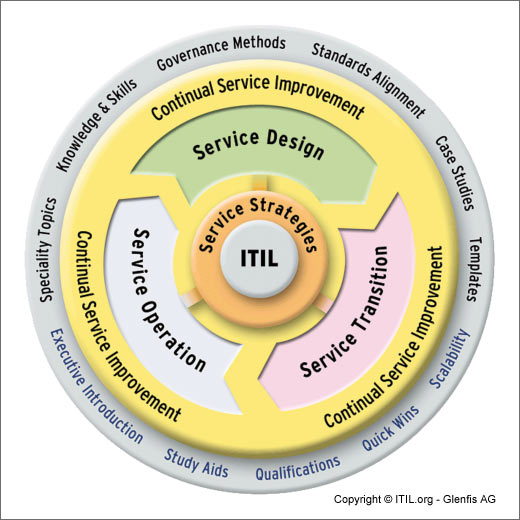
\includegraphics[width=0.50\textwidth]{Abbildungen/ITIL_Lebenszyklus}
	\caption[ITIL Service Lifecycle]{ITIL Service Lifecycle, Quelle: http://os.itil.org/osMedia/site/t1 
	media/JPEG/01\_itil\_imap.jpg}
	\label{fig:ITIL_Lebenyzyklus}
\end{figure}

\noindent
Auf alle Teilbeibereiche einzugehen, wäre zu zeitaufwendig, ist aber auch gar nicht nötig. Der Servicedesk ist nämlich Bestandteil der Service Operation und somit die richtige Anlaufstelle für die Begriffsklärung. \newline \enquote{Service Operation beschreibt den Abschnitt des Lebenszyklus, der von den Kunden primär wahrgenommen wird.}\footnote{Vgl. Ebel, N. (2008): ITIL® V3 Basis-Zertifizierung, S.439.} In der Service Operations-Phase werden die Prozesse und Funktionen beschrieben, die einen stabilen  und bestmöglich IT Service garantieren sollen. Bei dieser Verbindung von IT Organisation und Kunde wird besonders auf den Kunden eingegangen. Der Servicedesk ist hierbei \enquote{die zentrale Anlaufstelle, der Single Point of Contact (SPoC) zwischen Anwender und der IT-Organisation}\footnote{Vgl. Ebel, N. (2008): ITIL® V3 Basis-Zertifizierung, S.439.}. Wie der Name schon verrät, kommt der Anwender nur über diese Schnittstelle in Kontakt mit der IT. Hier werden Meldungen der Anwender üblicherweise erfasst, kategorisiert und eingetragen. Der Servicedesk ist nicht nur eine Kommunikationsunterstürzung, sondern bietet gleichzeitig eine Auskunft für bereits bekannte Probleme. Dadurch kann bei häufig auftretenden Service-Unterbrechungen schneller gehandelt werden. Auch Supportanfragen, Beschwerden, Verbesserungsvorschläge oder Änderungswünsche können in den Servicedesk eingetragen werden. Diese einzelnen Managementbereiche von ITIL v3 (Incident -, Problem -, Configuration -, Change -und Release Management) laufen im Servicedesk zusammen, sodass der Benutzer nicht mehr entscheiden muss, in welchen Bereich sein Problem/Vorfall eingeordnet werden muss. Das ist dann Aufgabe des Supports. Die nachfolgende Abbildung verdeutlicht dieses Vorgehen.

\begin{figure}[h!]
\centering
	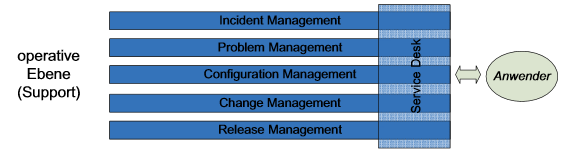
\includegraphics[width=0.75\textwidth]{Abbildungen/SPOC_2.png}
	\caption[Single Point of Contact]{Single Point of Contact, Quelle:http://edoc.hu-berlin.de/
	conferences/dfn2006/fischlin-roger-105/PDF/fischlin.pdf}
	\label{fig:ITIL_Lebenyzyklus}
\end{figure}

\subsection{Unterschied zu Helpdesk}

\noindent
Bei der Begriffsabgrenzung zwischen Helpdesk und Servicedesk ist Vorsicht geboten. In mehreren Quellen ist zu finden, dass Helpdesk (auch User-Help-Desk) lediglich ein veralteter Begriff für den Servicedesk sei.\footnote{Vgl. Victor, F./Günther, H. (2005): Optimiertes
IT-Management mit ITIL, S.24.}\footnote{Meier, A./Myrach, T, (2004): IT-Servicemanagement, S.26.} Im Internet heißt es Beispielsweise auf Wikipedia: \enquote{Der Artikel Helpdesk und Servicedesk überschneiden sich thematisch.}\footnote{https://de.wikipedia.org/wiki/Servicedesk, Stand 08.11.2013} In anderen Literaturquellen tritt der Begriff Helpdesk erst gar nicht auf oder wird dem Servicedesk gleichgesetzt\footnote{Vgl. Olbrich, A. (2008): ITIL Kompakt und verständlich, S.19.}. Im Zweifelsfall sollte man sich direkt auf das Buch ITIL Service Operation beziehen. In dem heißt es übersetzt unter dem Stichwort Help Desk:
\enquote{Eine Anlaufstelle für Anwender, um Incidents zu erfassen. Ein Help Desk ist in der
Regel eher technisch orientiert als ein Service Desk und stellt keinen Single Point
of Contact für die gesamte Interaktion bereit. Der Begriff „Help Desk“ wird häufig
auch als Synonym für Service Desk verwendet.} \footnote{Vgl. Cannon, D./Wheeldon, D. (2007): Service Operation, S. 233. Übersetzung entnommen aus: Ebel, N. (2008): ITIL® V3 Basis-Zertifizierung, S. 699.} \newline
In den weiteren Ausführungen gilt deshalb der Helpdesk als Synonym für den Servicedesk. Auch im Punkt 2.3.3 \enquote{Vergleich verschiedener Servicedesk-Lösungen} wird diese Begriffsüberschneidung bzw. Gleichbedeutung noch einmal deutlich.



\subsection{Anforderungen eines Servicedesk}

\subsubsection{Aufgaben}
\noindent
Im folgenden sollen die wichtigsten Aufgaben eines Servicedesk aus Sicht der ITIL v3 erläutert werden. Hierfür wird zunächst stichpunktartig die Kernaussage festgehalten, um sie anschließend zu erläutern. Dabei beziehen sich die Kernaussagen auf der Ausarbeitung Olbrichs aus \enquote{ITIL Kompakt und verständlich}
\footnote{Olrich, A. (2008): ITIL kompakt und verständlich, S.19 f.}
und sind eine leicht abgewandelte Form vom ITIL v3 Band Service Operation \footnote{Vgl. Cannon, D./Wheeldon, D. (2007): Service Operation, S. 110.}

\begin{itemize}
\item \enquote{Einheitlichen, zentralen Kommunikationsschnittstelle (SPoC) mit konkreten Ansprechpartner}
\end{itemize}
\noindent
Der Kunde hat mehrere Möglichkeiten den Support zu kontaktieren. Schreibt der Kunde eine E-Mail an den Support, könnte diese ausgewertet und den Servicedesk eingetragen werden. Ebenso könnte er selbst einen Eintrag über ein Web-Frontend erstellen. Oder aber der Support erstellt einen solchen Eintrag im Servicedesk, wenn der Kunde zum Telefon greift. Es ist aber Voraussetzung, dass eine einheitliche und zentrale Kommunikationsschnittstelle bereitgestellt wird.


\begin{itemize}
\item \enquote{Aufnahme, Dokumentation und Auswertung aller Vorfälle}
\end{itemize}
\noindent
Wenn alle Vorfälle ordnungsgemäß aufgenommen und dokumentiert wurden, kann schneller reagiert werden, wenn sich ein Problem wiederholt. Dass alle Vorfälle auch ausgewertet werden sollten, ist verständlich und kann eventuell dazu beitragen, Folgeprobleme frühzeitig zu erkennen.

\begin{itemize}
\item \enquote{Überwachung, Nachverfolgung und Eskalation von laufenden
Supportvorgängen. Frühzeitiges Erkennen von
Bedürfnissen und Problemsituationen}
\end{itemize}
\noindent
Wie im Punkt zuvor erwähnt können Probleme frühzeitig erkannt werden, indem Vorfälle genauestens ausgewertet werden. Das ist aber längst nicht die einzige Möglichkeit, Bedürfnisse der Kunden zu erkennen. Gute Mittel für vorausschauende Handlungen sind  bspw. Monitoring-Systeme oder log-Files. Sie liefern technische Informationen, die - nach einer Auswertung - Aufschluss über die aktuelle Lage des Kunden geben und in den Servicedesk integriert werden könnten.


\begin{itemize}
\item \enquote{Überprüfung der Einhaltung des Dienstleistungsgegenstands
anhand von Service-Level-Agreements}
\end{itemize}
\noindent
Mithilfe des Servicedesks kann kontrolliert werden, ob die vereinbarten Leistungen zwischen Auftraggeber und Beauftragter eingehalten wurden, wenn alle Vorfälle dokumentiert wurden.

\begin{itemize}
\item \enquote{Reporting – Beauskunftung gegenüber den Usern (Kunden)
und dem Management. Informationen über den aktuellen
Status von Vorgängen, geplanten Änderungen und
verschiedenen Nutzungsmöglichkeiten}
\end{itemize}
\noindent
Der Servicedesk dient außerdem dazu, stets mit dem Kunden im Kontakt zu stehen. So können Information an den Kunden weitergeleitet oder auf der anderen Seite aktuelle Vorgänge, Status etc. des Kunden verfolgt und analysiert werden. 

\begin{itemize}
\item \enquote{Überprüfen der Kundenzufriedenheit, Stärkung der Kundenbeziehung.
Kontaktpflege. Aufspüren neuer Geschäftschancen}
\end{itemize}
\noindent
Nicht zuletzt kann der Servicedesk auch als Instrument für einen ständigen Kontakt zum Kunden eingesetzt werden. Der Kunde hat dadurch den Eindruck, permanent mit der Support und somit der Firma verbunden zu sein. Das kann das Verhältnis zum Kunden stärken oder gar neue Geschäftsmöglichkeiten eröffnen.\\


\subsubsection{Kategorien}

\noindent
Grundsätzlich gibt es drei Kategorien bezüglich der Architektur eines Servicedesks:

\begin{itemize}
\item Lokaler Servicedesk
\item Zentraler Servicedesk
\item Virtueller Servicdesk
\end{itemize}

\noindent
Der lokale Servicedesk zeichnet sich dadurch aus, dass er innerhalb eines Bereiches selbständig agiert. Mehrere Unternehmensstandorte oder verschiedene Bereiche eines Unternehmens haben jeweils einen eigenen Servicedesk. Dieser kann präzise auf die Probleme und Prozesse vor Ort angepasst werden. Jedoch gestaltet sich eine Zusammenarbeit mehrere Bereiche gerade wegen dieser individuellen Servicedesks schwierig. \\

\noindent
Beim zentralen Servicedesk ist diese bereichsübergreifende Zusammenarbeit keine Hürde, da es einen Servicedesk gibt, der für alle Bereiche eine gleichmäßige Zuständigkeit besitzt. Die Prozesse und Abläufe aller Benutzer sind hier identisch. Zwar sind die Kommunikationsmöglichkeiten hier sehr umfangreich, jedoch wächst die Informationsmenge rasant an. Eine kundennahe Betreuung wird durch den hohen Organisationsumfang deutlich erschwert. \\

\noindent
Bei der Kompromisslösung dieser beiden Architekturmodellen stößt man auf den virtuellen Servicedesk. Die Informationseingabe der Benutzer kann durchaus an verschiedenen Standorten erfolgen ganz wie beim lokalen Servicedesk. Doch alle Daten werden gesammelt und zentral verwaltet, was dem zentralen Servicedesk entspricht. Entscheidend ist hierbei, dass es einheitliche Prozesse und Abläufe an den einzelnen Standorten geben muss. Individuelle Servicedesks wären zu aufwendig in der Verwaltung. Auch so ist der Ressourcen -und Organisationsaufwand gegenüber den anderen Modellen enorm und bedarf guter Planung. \footnote{Vgl. Olbrich, A. (2008): ITIL kompakt und verständlich, S.21.} \footnote{Vgl. Cannon, D./Wheeldon, D. (2007): Service Operation, S. 111 f.} \\


\subsection{Vergleich verschiedener Servicedesk-Lösungen}

\noindent
Nach diesem sehr theoretischem Ansatz die Anforderungen eines Servicedesks zu klären, wird nun auf Beispiele in der Praxis eingegangen. Wichtig sind dabei nicht Kriterien wie das äußere Erscheinungsbild oder die Kosten. Ziel soll es sein durch einen Vergleich gängiger Softwarelösungen, Verbesserungsmöglichkeiten der eigene Servicedesk-Funktionalität in GEBman10 zu ermitteln. Dabei wird auf die drei folgenden Punkte Wert gelegt:

\begin{itemize}
\item Funktionalität:\\
		Die Funktionalität ist wohl das fundamentalste Kriterium. Hier ist entscheidend, welche 			
		Möglichkeiten dem Benutzer gegeben werden bspw. Meldungen/Tickets anzulegen, zu 
		zuweisen, zu suchen oder zu filtern. Wichtig ist aber auch, welche Informationen in welcher 
		Darstellungsform erhalten sind (Diagramme etc.) und welche Daten erfasst werden müssen 
		bzw. können.\\
		 
\item Bedienbarkeit:\\
		Aus diesem Blickwinkel wird untersucht, welche Bedienelemente zur Verfügung stehen. Eine	
		Bewertung nach intuitiver Bedienbarkeit ist schwierig vorzunehmen, da das immer eine
		subjektive Ansicht enthält.\\
		
\item Anpassbarkeit:\\
		Inwieweit kann man bspw. die grafische Oberfläche vom Benutzer geändert und auf die 
		eigenen Bedürfnisse angepasst werden.\\		
\end{itemize}


%hier sollte noch ein abschließender Satz hin

\noindent
Nach den Recherchen auf mehreren Review und Ranking Websites zum Thema Service Desk / Help Desk, sind drei Softwarelösungen wiederholt erwähnt und gut bis sehr gut bewertet worden.\footnote{siehe Literaturverzeichnis}Diese drei webbasierten Anwendungen werden nun kurz vorgestellt, um sie anschließend ihre Stärken und zu ermitteln.

\begin{itemize}
\item Freshdesk:\\
		\\
		 
\item Desk.com:\\
		\\
		
\item Zendesk:\\
		\\		
\end{itemize}

\noindent
Aktuelle benutzt der Support von der KMS Computer GmbH die Software SysAid für den Service Desk. Durch eine Vielzahl von Einträgen und Erfahrungen der Mitarbeiter im Support, ist es sinnvoll auch diese Anwendung mit in den Vergleich einfließen zu lassen.

\begin{itemize}
\item Freshdesk:\\
		\\
\end{itemize}	


\noindent
Vgl. IT Notfallmanagement unter Incident Management
\newpage

%-------------------------------------------------------------------------------------------------------
%					3	Servicedesk in GEBman10
%-------------------------------------------------------------------------------------------------------

% !TEX root = Bachelorarbeit_Paul_Zilewitsch.tex

\section{Der Service Desk in GEBman10}

\subsection{Aktuelle Umsetzung}
\noindent
Der Service Desk in GEBman10 ist ein eigenständiges Modul. Im Dashboard dieses Moduls werden alle Meldungen angezeigt, die erstellt wurden. Dabei spielt der Status dieser Meldungen zunächst keine Rolle. Der Benutzer erhält mittels eines Diagramms direkt einen Einblick auf die Meldungen innerhalb einer Woche. Unterteilt wird hierbei in eingegangene Meldungen, Meldungen die in Bearbeitung sind, unbearbeitete Meldungen und fertige Meldungen. Ein zweites Diagramm veranschaulicht die Verweildauer einer Meldung, in dem die Zeit zwischen dem unbearbeiteten Zustand und dem der Bearbeitung protokolliert wird. Unter den beiden Diagrammen finden sich alle Fakten noch einmal in Form von Zahlen wieder. Der Benutzer hat nun direkt die Möglichkeit für eine Detailansicht einer oder mehrerer Meldung, eine neue Meldung anzulegen, eine Filterung der Meldung vorzunehmen oder die Einstellungen anzupassen. Der Aufbau wird in der Abbildung XX deutlicher. 

\begin{figure}[h!]
\centering
	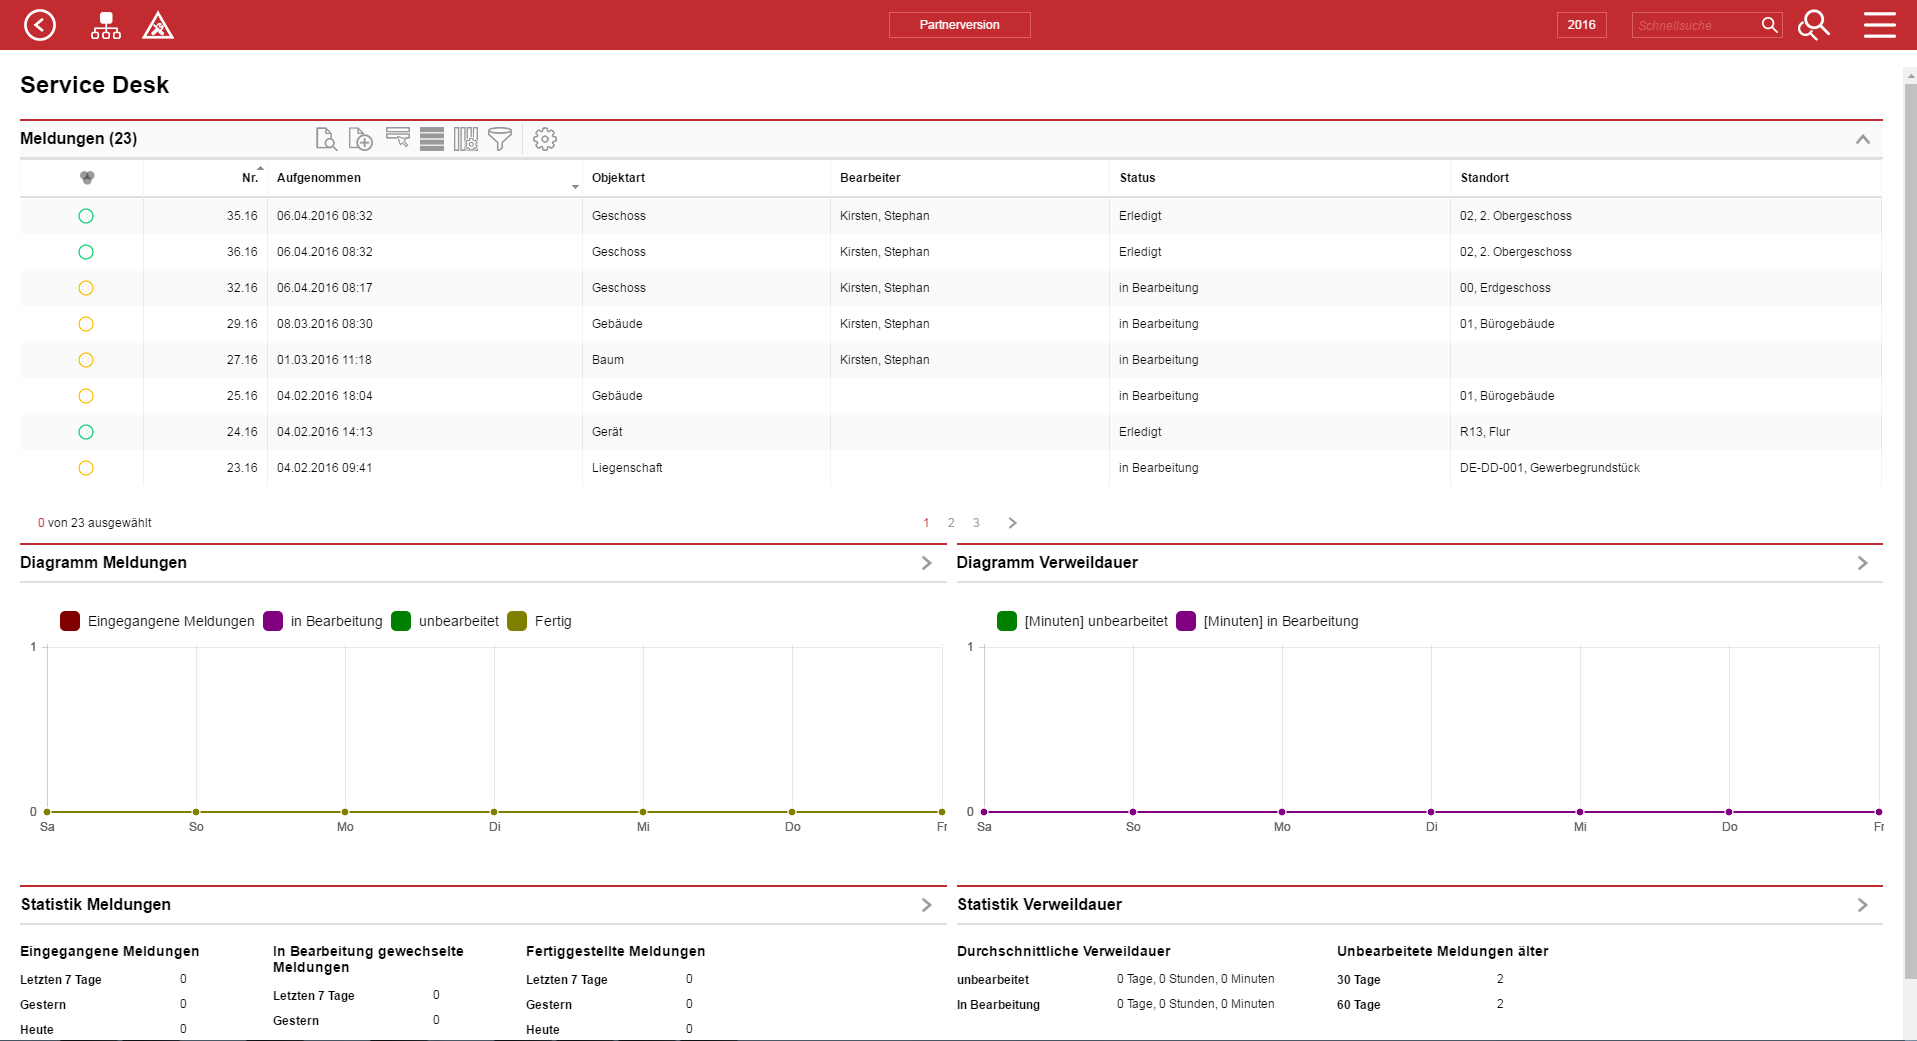
\includegraphics[width=0.75\textwidth]{Abbildungen/GEBman_Service_Desk_Dashboard}
	\caption[GEBman10 Service Desk Dashboard]{GEBman10 Service Desk Dashboard, Quelle: 
	GEBman10}
	\label{fig:ITIL_Lebenyzyklus}
\end{figure}


\subsection{Anforderungen der Erweiterung}

\noindent
Qualität ist ein Maß für das Erfüllen von Anforderungen. Die Qualität des Service Desk kann deshalb nur gesichert werden, wenn die Anforderungen möglichst genau definiert werden. Zu den zu erfüllen Anforderungen sollte aber noch festgehalten werden, welche Anforderungen nicht erfüllt werden sollen. Letzteres wird häufig nicht beachtet, ist jedoch ein wesentlicher Schritt für das Sicherstellen der Anforderungen. \footnote{Vorlesungsreihe Qualitätsmanagement: Hans-Jörg Günther, 6.Semester}

\colorbox{red}{hier muss noch einmal auf alle Punkte von 2. eingegangen werden, um abzugrenzen, was eine Anforderung ist und was eben nicht! }
\newpage

%-------------------------------------------------------------------------------------------------------
%					4	Microsoft Exchange Server
%-------------------------------------------------------------------------------------------------------

% !TEX root = Bachelorarbeit_Paul_Zilewitsch.tex
\section{Microsoft Exchange Server}

\subsection{Grundlagen}
\noindent 
Der  Microsoft Exchange Server ist eine serverseitige Anwendung, die den Nachrichtenaustausch und die Zusammenarbeit im Unternehmen erleichtern soll.\footnote{Joos, T. (2013): Microsoft Exchange Server 2013, S.26.} Im Juni 1996 wurde die erste Version von Microsoft Exchange veröffentlicht. Sie löste das Mailsystem MS Mail ab, da dieses für einen Gebrauch mit über 500 Postfächern nicht ausgelegt und somit für größere Unternehmen nicht mehr sinnvoll war. Dieser Wechsel der Software wurde passend durch den Namen Exchange beschrieben, da es so viel heißt wie \enquote{Austausch}.\footnote{Vgl. Übersetzer}
Ziel des Microsoft Exchange Servers ist es, Nachrichten zu verarbeiten und zu verwalten. Obwohl Exchange ein Mailserver ist, können neben E-Mails auch Termine angelegt oder Aufgaben vergeben werden. Somit wäre es denkbar, Exchange als zentrale Anlaufstelle der Unternehmenskommunikation einzusetzen.

\noindent 
Microsoft Exchange ist klar in den Bereich Groupware einzuordnen. Gropuware-Software wird vor allem zur Unterstützung der internen als auch der externen Unternehmenskommunikation genutzt. Ellis, Gibbs und Rein beschreiben die bekannteste Form von Groupware als ein 
\enquote{computer-based message system, which supports the asynchronous exchange of textual messages between groups of users}\footnote{Ellis, C. A./Gibbs, S. J./Rein, G. L. (1991): Groupware - Some Issues and Experiences. Communications of the ACM, 34(1), S. 38-58.}. Also ein Computersystem für den asynchronen Austausch von von Textnachrichten innerhalb einer Gruppe. Meistens sind dies Arbeitsgruppen im Unternehmensumfeld. Mircosoft Exchange erfüllt dieses Kriterium. Vorausgesetzt die Benutzer verfügen über eine Client-Software.

\noindent
Um auf die Inhalte des Microsoft Exchange Servers zugreifen zu können, benötigt jeder Benutzer eine Client-Software. Verwaltung des Postfaches, Zugriff auf öffentliche Ordner und natürlich auch Empfangen und Senden von E-Mails sind die Hauptziele einer Client-Software. Im Anhang auf Seite~\pageref{Exchange Verbindung} findet man eine Abbildung, die eine umfassende Übersicht verschiedener Clients darstellt. Diese Übersicht ist nicht Vollständigkeit, bildet aber dennoch die am häufigsten verwendeten Client-Systeme ab.

\noindent
Am bekanntesten ist sicher der Microsoft Outlook-Client. Aus diesem Grund wird die Verbindung eines Clients mit dem Exchange Server am Beispiel des Outlook-Clients erläutert. Outlook kommuniziert nach dem RPC-Prinzip mit dem Exchange Server. Die Variante RPC über TCP/IP  gilt zwar seit Exchange 2013 als veraltet, ist aber für das nähere Verständnis durchaus wichtig, da alle Weiterentwicklungen RPC im Hintergrund weiter nutzen. RPC bedeutet "Remote Procedure Call" und wird verwendet, um eine Verbindung zu einem Dienst eines Servers herzustellen. Als Übertragungsprotokoll fungiert TCP/IP (Transfer Control Protocol/Internet Protocol).\footnote{Vgl. http://www.msxfaq.de/verschiedenes/rpc.htm}Um die Kommunikation von RPC über TCP/IP zu verstehen, ist die nachfolgende Abbildung hilfreich.

\begin{figure}[h!]
\centering
	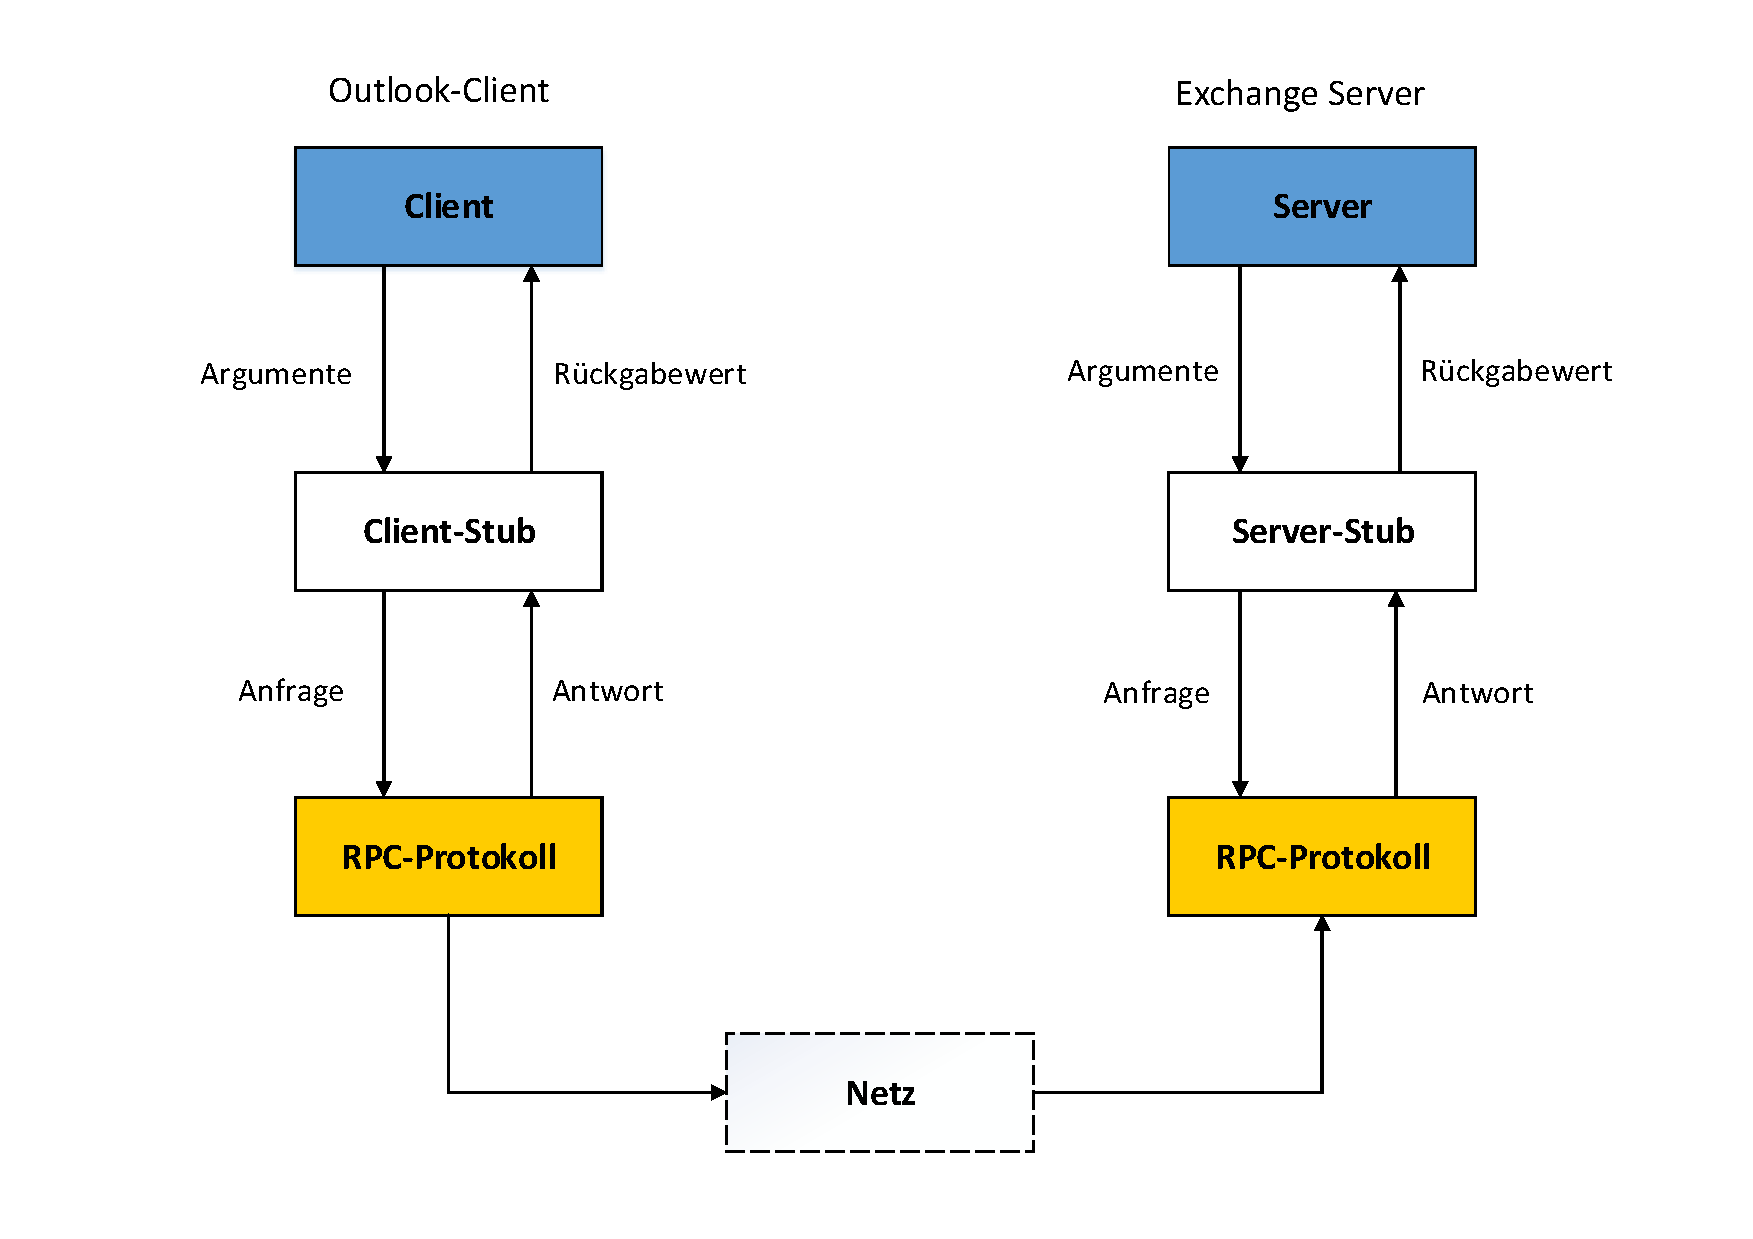
\includegraphics[width=0.60\textwidth]{Abbildungen/RPC_TCP}
	\caption[Aufbau einer klassischen RPC Verbindung]{Aufabu einer klassischen RPC Verbindung,    in Anlehnung an:\\https://technet.microsoft.com/de-de/library/e8feb37e-f3a9-4f26-bed0-6583d8a110ed}
	\label{fig:RPC_TCP}
\end{figure}

\noindent 
Der Client ruft eine Prozedur mit spezifischen Argumenten (Eingabeparameter) auf. Der Client-Stub aktiviert eine gleichnamige Prozedur und wandelt die Argumente in ein plattformunabhängiges Datenformat um. Die Daten werden dann über das Netz mithilfe des TCP/IP-Protokolls an den Server geschickt. Dort erhält der Server-Stub die Anfrage und wandelt die Argumente in das lokale Format des Servers um. Nun ruft der Server die gewünschte Prozedur mit den Eingabeparametern auf und der Rückgabewert kehrt in den Server-Stub zurück. Nach einer erneuten plattformunabhängigen Umwandlung der Datenformate, wird die Antwort an den Client-Stub geschickt. Im letzten Schritt erhält der Client die in das lokale Format umgewandelte Antwort (Rückgabewerte) auf seine Anfrage.\footnote{Vgl. Schneider, U. (2012): Taschenbuch der Informatik, S.406 f.}

\noindent 
Ab Exchange 20013 wird der Datenaustausch zwischen dem Outlook-Client und dem Exchanger Server standardmäßig über RPC/HTTP (auch Oulook Anywhere genannt) geregelt. Wie der Name schon vermuten lässt, läuft die gesamte Kommunikation bei dieser Variante über HTTP bzw. HTTPS. Somit kann über das Internet auf den Exchange Server zugegriffen werden. Outlook Anywhere ist besonders für Mitarbeiter geeignet, die von zu Hause auf ihr Exchange-Postfach zugreifen möchten, da sie sich nicht im Unternehmensnetzwerk befinden müssen.\footnote{Vgl. Joos, T. (2013): Microsoft Exchange Server 2013, S.33, S.254.} 

\begin{figure}[h!]
\centering
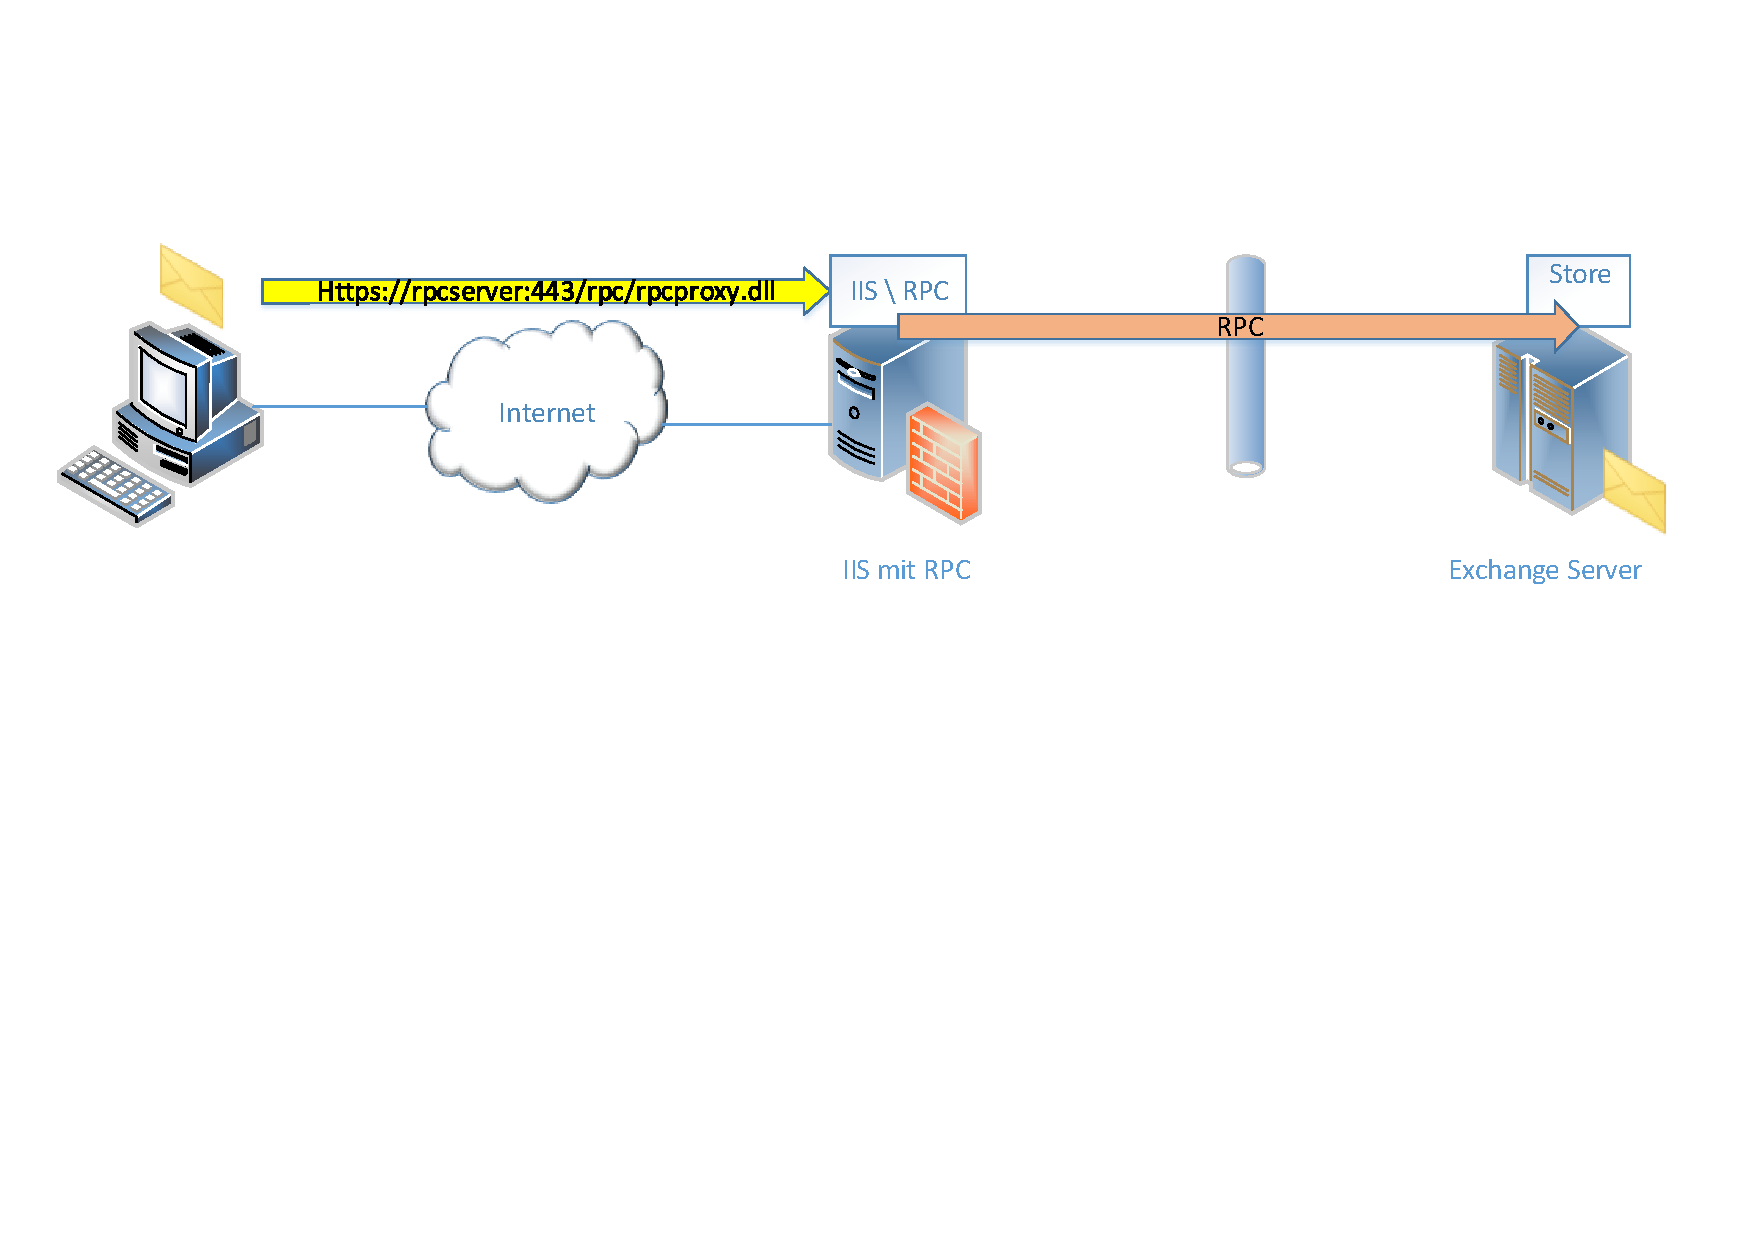
\includegraphics[width=0.65\textwidth]{Abbildungen/RPC_HTTP}
	\caption[RPC over HTTP Prinzip]{RPC over HTTP Prinzip,  in Anlehnung an:http://
	www.msxfaq.de/clients/oagrundlagen.htm}
	\label{fig:RPC_HTTP}
\end{figure}

\noindent
In der Abbildung \ref{fig:RPC_HTTP} sieht man deutlich, dass der Outlook-Client über HTTPS mit dem IIS kommuniziert, auf dem ein virtuelles RPC-Verzeichnis existiert. Der IIS ist eine Microsoft-Webserverplattform, die Webanwendungen und Dienste bereitstellen und verwalten kann.\footnote{Vgl. Volodarsky, M./Cheah, B./Londer, O./Hill,B./Schofield, S./Aguilar Mares,C./Meyer,K./ Microsoft IIS Team (2009):Microsoft
Internetinformations-dienste (IIS) 7.0 – Die technische Referenz, S.3.} Der IIS wiederum, baut über einen RPC-Proxy eine Verbindung mit dem Exchange Server auf. Wichtig ist hierbei, dass die Kommunikation des Clients sich auf HTTP oder HTTPS beschränkt.\footnote{Vgl. http://www.msxfaq.de/clients/oagrundlagen.htm}


\subsection{Exchange Web Services}
\noindent
Die Grundlagen von Mircosoft Exchange Server sind geklärt. Doch wie können nun Programmierer über Quellcode auf den Exchange Server zugreifen. Hierfür hat Mircosoft im Laufe der Jahre eine Reihe von Programmierschnittstellen bereitgestellt. Eine Schnittstellen zur Anwendungsprogrammierung wird als API (englisch application programming interface) bezeichnet. Es ist nicht nötig, alle Programmierschnittstellen zu erläutern, da eine Vielzahl der APIs keine Verwendung mehr finden oder nicht mehr unterstützt werden. Zu Informationszwecken befindet sich jedoch im Anhang auf Seite~\pageref{API_1} eine Übersicht einiger Programmierschnittstellen ab dem Jahr 1992. Ab Exchange 2007 setzt Microsoft immer mehr auf den Exchange Web Services (kurz EWS) als Programmierschnittstelle und baut diese seitdem weiter aus.
\footnote{http://www.msxfaq.de/code/ews.htm}
Redmond schreibt im Handbuch Exchange 2010: 
\enquote{Abgesehen von Windows PowerShell liegt der Schwerpunkt für die meisten Entwickler jetzt auf der API EWS (Exchange-Webdienste), die in Exchange Server 2007 eingeführt wurde.}\footnote{Vgl. Redmond, T. (2011): Microsoft Exchange Server 2010, S.634.}
Er macht deutlich, dass EWS die erste Anlaufstelle für Entwickler ist. Eine weitere Programmierschnittstelle namens REST API erschien 2015 mit Office 365 .Der REST API wird aber keine weitere Beachtung geschenkt, da sie lediglich in der Office 365-Umgebung Anwendung findet.
\footnote{https://msdn.microsoft.com/de-de/library/office/dn776319\%28v=exchg.150\%29.aspx}


\subsubsection{Funktionsweise}
\noindent
Standardmäßig bildet das Simple Object Access Protocol (kurz SOAP) eine Grundlage für Web-Services. Schneider beschreibt SOAP als \enquote{ein RPC-Mechanismus, bei dem die übertragenen Daten im XML-Format codiert werden.}\footnote{Vgl. Schneider, U. (2012): Taschenbuch der Informatik, S.407.}
Schill und Springer schreiben genauer: \enquote{Das objektorientierte Kommunikationsprotokoll SOAP ermöglicht die Kommunikation zwischen heterogenen Diensten unter interner Nutzung
des Hypertext Transfer Protocol (HTTP) und mit Kodierung der Parameter in der eXtensible Markup Language (XML).}\footnote{Vgl. Schill, A./Springer,T. (2012): Verteilte Systeme. S.69.}
Auch die Exchange Web Services funktionieren nach diesem Prinzip.\footnote{Vgl. https://msdn.microsoft.com/en-us/library/office/dd877045\%28v=exchg.140\%29.aspx} 
 
\noindent
Mit Exchange 2007 wurde erstmals der Exchange Web Services  bereitgestellt und löste nach und nach andere APIs ab. Die nachfolgende Abbildung zeigt, wie sich EWS seit 2007 entwickelt hat.

\begin{figure}[h!]
\centering
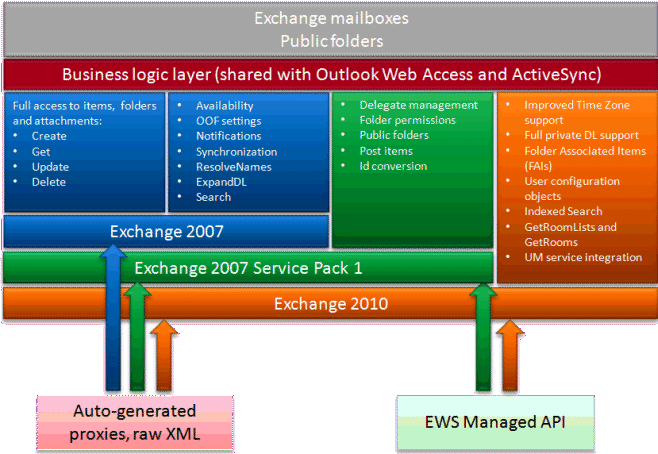
\includegraphics[width=0.65\textwidth]{Abbildungen/EWS_Funktionsumfang.png}
	\caption[EWS Funktionsumfang]{EWS Funktionsumfang, Quelle: http://www.msxfaq.de/code/
	ews.htm}
	\label{fig:EWS_Funktionsumfang}
\end{figure}

\noindent
EWS bietet einen großen Funktionsumfang und ist somit eine hervorragende Möglichkeit auf die Daten des Exchange Servers zuzugreifen. Aus diesem Grund haben sich die Entwickler der KMS Computer GmbH für diese Programmierschnittstelle entschieden.

\subsubsection{Derzeitige Verwendung in GEBman10}
\noindent
GEBman10 unterstützt Exchange Server 2007, Exchange Server 2007\_SP1, Exchange Server 2010 sowie Exchange Server 2010\_SP1. 
In Groupware kann....Auswahl getroffen werden. Die Implementation erfolge über EWS bzw. mit der Hilfe von der Microsoft Exchange Web Services Managed API 2.2.

Diese bereits vorhandenen Funktionalitäten werden als Grundlage für die folgenden Konzipierung und anschließende Implementierung genutzt. 

\newpage

%-------------------------------------------------------------------------------------------------------
%					5	Konzipierung
%-------------------------------------------------------------------------------------------------------

% !TEX root = Bachelorarbeit_Paul_Zilewitsch.tex
\section{Konzipierung}
\subsection{Analyse aus Kapitel 1 und Kapitel 2 (UML-Diagramme etc.)}
\subsection{Zielsetzung}
\subsection{Sicherheitsaspekte}
\noindent
Immer wieder vernachlässigen Entwickler die Sicherheit ihrer Implementierungen. Das liegt meistens an mangelnder Zeit, da Releases einen festen Zeitplan verfolgen, den es einzuhalten gilt. Es kann aber auch sein, dass die Implementierung nicht aus dem Blickwinkel der Sicherheit betrachtet wird. "Hauptsache es funktioniert erst einmal", wird dann häufig als Argument genutzt. Natürlich hat das wenig mit Sicherheit zu tun. Dabei können es Entwickler mit wenig Aufwand, Angreifern deutlich schwerer machen. Deswegen werden im nachfolgendem zwei Sicherheitsprobleme für die Umsetzung des Konzepts in GEBman 10 besprochen. Die Abbildung XX zeigt zwei kritische Bereiche, die genauer erläutert werden müssen.

\begin{figure}[h!]
\centering
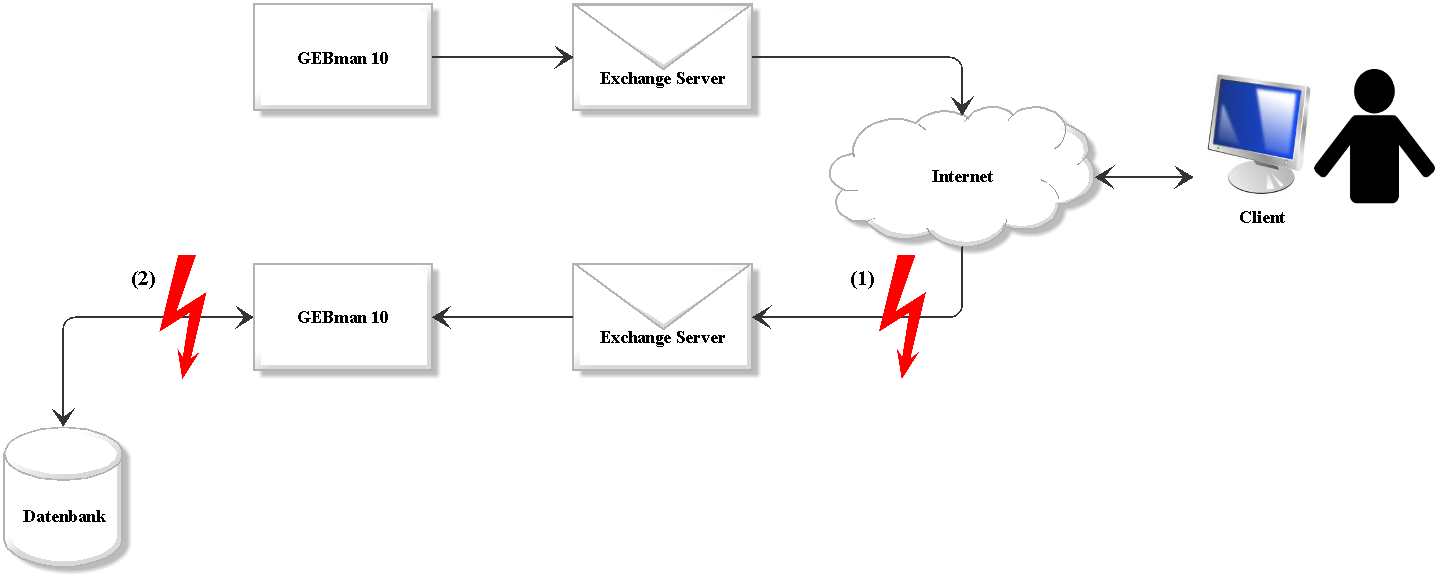
\includegraphics[width=0.85\textwidth]{Abbildungen/Sicherheitsprobleme.png}
	\caption[Sicherheitsprobleme]{Sicherheitsprobleme, Quelle:eigene Darstellung}
	\label{fig:Sicherheitsprobleme}
\end{figure}

\noindent
Der rechte rote Blitz - gekennzeichnet mit der (1) - symbolisiert das erste Problem.

\noindent
Beim zweiten roten Blitz der Abbildung XX - gekennzeichnet mit der (2) - wird uns die Arbeit nicht wie beim ersten kritischen Bereich abgenommen. GEBman 10 synchronisiert in regelmäßigen Abständen die Nachrichten vom hinterlegten Exchange Server. Entsprechend ihrer ID werden die Nachrichten in die Datenbank von GEBman 10 gespeichert. Nun könnte ein Angreifer beispielsweise versuchen, in den Mail-Body versteckte SQL -Anweisungen oder JavaScript-Code einzuschleusen. Werden die SQL-Anweisungen in die Datenbank geschrieben, ohne sie vorher zu validieren, könnte der Angreifer Informationen über Daten in der Datenbank erlangen. Im schlimmsten Fall könnte er sie zerstören. Diese Angriffstmethode nennt sich SQL-Injection und zielt darauf ab, die normalen SQL-Statements mittels Sonderzeichen zu manipulieren. Selbst einfache Zeichen wie "--" können bewirken, dass alles, was hinter den beiden Bindestrichen steht, ignoriert wird. In T-SQL sind die beiden Bindestriche das Zeichen für einen Kommentar.
\noindent
Bei JavaScript-Code haben wir ein ähnliches Problem mit bestimmten Zeichen. Wird zum Beispiel die einfache Zeichenfolge "<script>alert('hallo')<script>" in die Datenbank geschrieben, passiert ersst einmal gar nichts. Die SQL-Statements werden hierdruch nicht manipuliert. Doch wird diese Zeichenfolge beispielsweise als Antwort auf eine Meldung geladen, erkennt der Browser möglicherweise JavaScript-Code anstatt einfachen Text. Das hat in unserem Beispiel zur Folge, dass der Browser eine kleine Nachricht meldet (siehe Abbildung).
Auch hier muss vor dem Einfügen der Zeichenfolge, eine Validierung vollzogen werden. Welche Zeichen genau gefiltert werden müssen, wird im Punkt 5 Umsetzung erläutert. Man sollte sich jedoch nicht darauf verlassen, dass die Schutzmechanismen des Microsoft Exchange Servers alle Zeichen und Zeichenfolgen als Bedrohung erkennen. Zeichen wie "--" oder ">" können durchaus im normalen Schriftverkehr gebräuchlich sein.
\noindent
Es gibt für Angreifer noch mehr Angriffsmöglichkeiten beispielsweise zwischen Client und Internet/Server über Man-in-the-Middle etc.. Darauf soll aber in dieser Arbeit nicht weiter eingegangen werden, da das ein sehr umfangreiches Thema ist und eine eigenständige Bachelorarbeit bilden könnte. Eins sollte jedem klar sein: Hat ein Cracker genügend Zeit und Ressourcen, ist ein System, das über das Internet kommuniziert, äußert schwer vollkommen zu sichern. 
\noindent
Durch die Analyse aus Punkt 2 und Punkt 3 konnte ein genaues Ziel gesetzt werden. Die Funktionsweise der Exchange Web Services sind geklärt und auch Sicherheitsaspekte wurden berücksichtigt. Die Konzipierung ist somit abgeschlossen und er Implementierung steht nichts mehr im Wege.

\newpage

%-------------------------------------------------------------------------------------------------------
%					6	Ummsetzung
%-------------------------------------------------------------------------------------------------------

% !TEX root = Bachelorarbeit_Paul_Zilewitsch.tex
\section{Umsetzung}
https://www.microsoft.com/en-us/download/details.aspx?id=42951

hier die Managed API herunterladen
\subsection{Erweiterung des bestehenden Service Desk Moduls}
\subsection{Erläuterung der wichtigsten Klassen und Methoden}
\subsection{Fehlschläge/Erfahrungen}
\newpage

%-------------------------------------------------------------------------------------------------------
%					7	Fazit
%-------------------------------------------------------------------------------------------------------

% !TEX root = Bachelorarbeit_Paul_Zilewitsch.tex
\section{Fazit}
\subsection{Erweiterungsmöglichkeiten}
\subsection{Schlussbemerkung}
\newpage

%-------------------------------------------------------------------------------------------------------
%					Anhangsverzeichnis
%-------------------------------------------------------------------------------------------------------
\addsec{Anhangsverzeichnis} %vergebe keine Kapitelnummer

\newpage

%-------------------------------------------------------------------------------------------------------
%					8 Anhang
%-------------------------------------------------------------------------------------------------------

\addsec{Anhang} %vergebe keine Kapitelnummer
% !TEX root = Bachelorarbeit_Paul_Zilewitsch.tex
\begin{flushright}
Anhang 1\\
Blatt 1\\
\end{flushright}

\noindent Einige Exchange Verbindungen
\begin{flushleft}
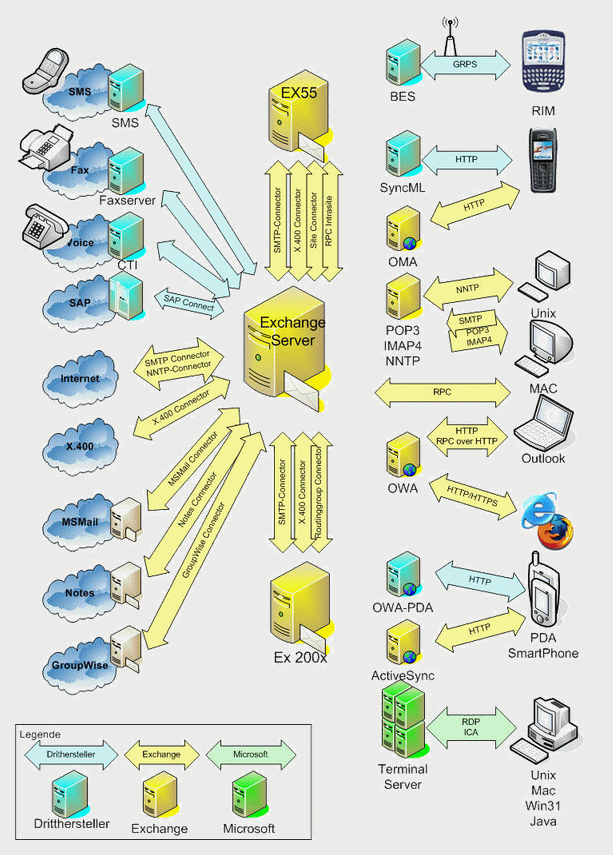
\includegraphics[width=0.65\textwidth]{Abbildungen/Exchange_Verbindungen.png}
\end{flushleft}
\label{Exchange Verbindung}
\noindent Quelle: http://www.msxfaq.de/basics/excomm.htm

\newpage

\begin{flushright}
Anhang 2\\
Blatt 2\\
\end{flushright}

\noindent Übersicht verschiedener APIs
\begin{flushleft}
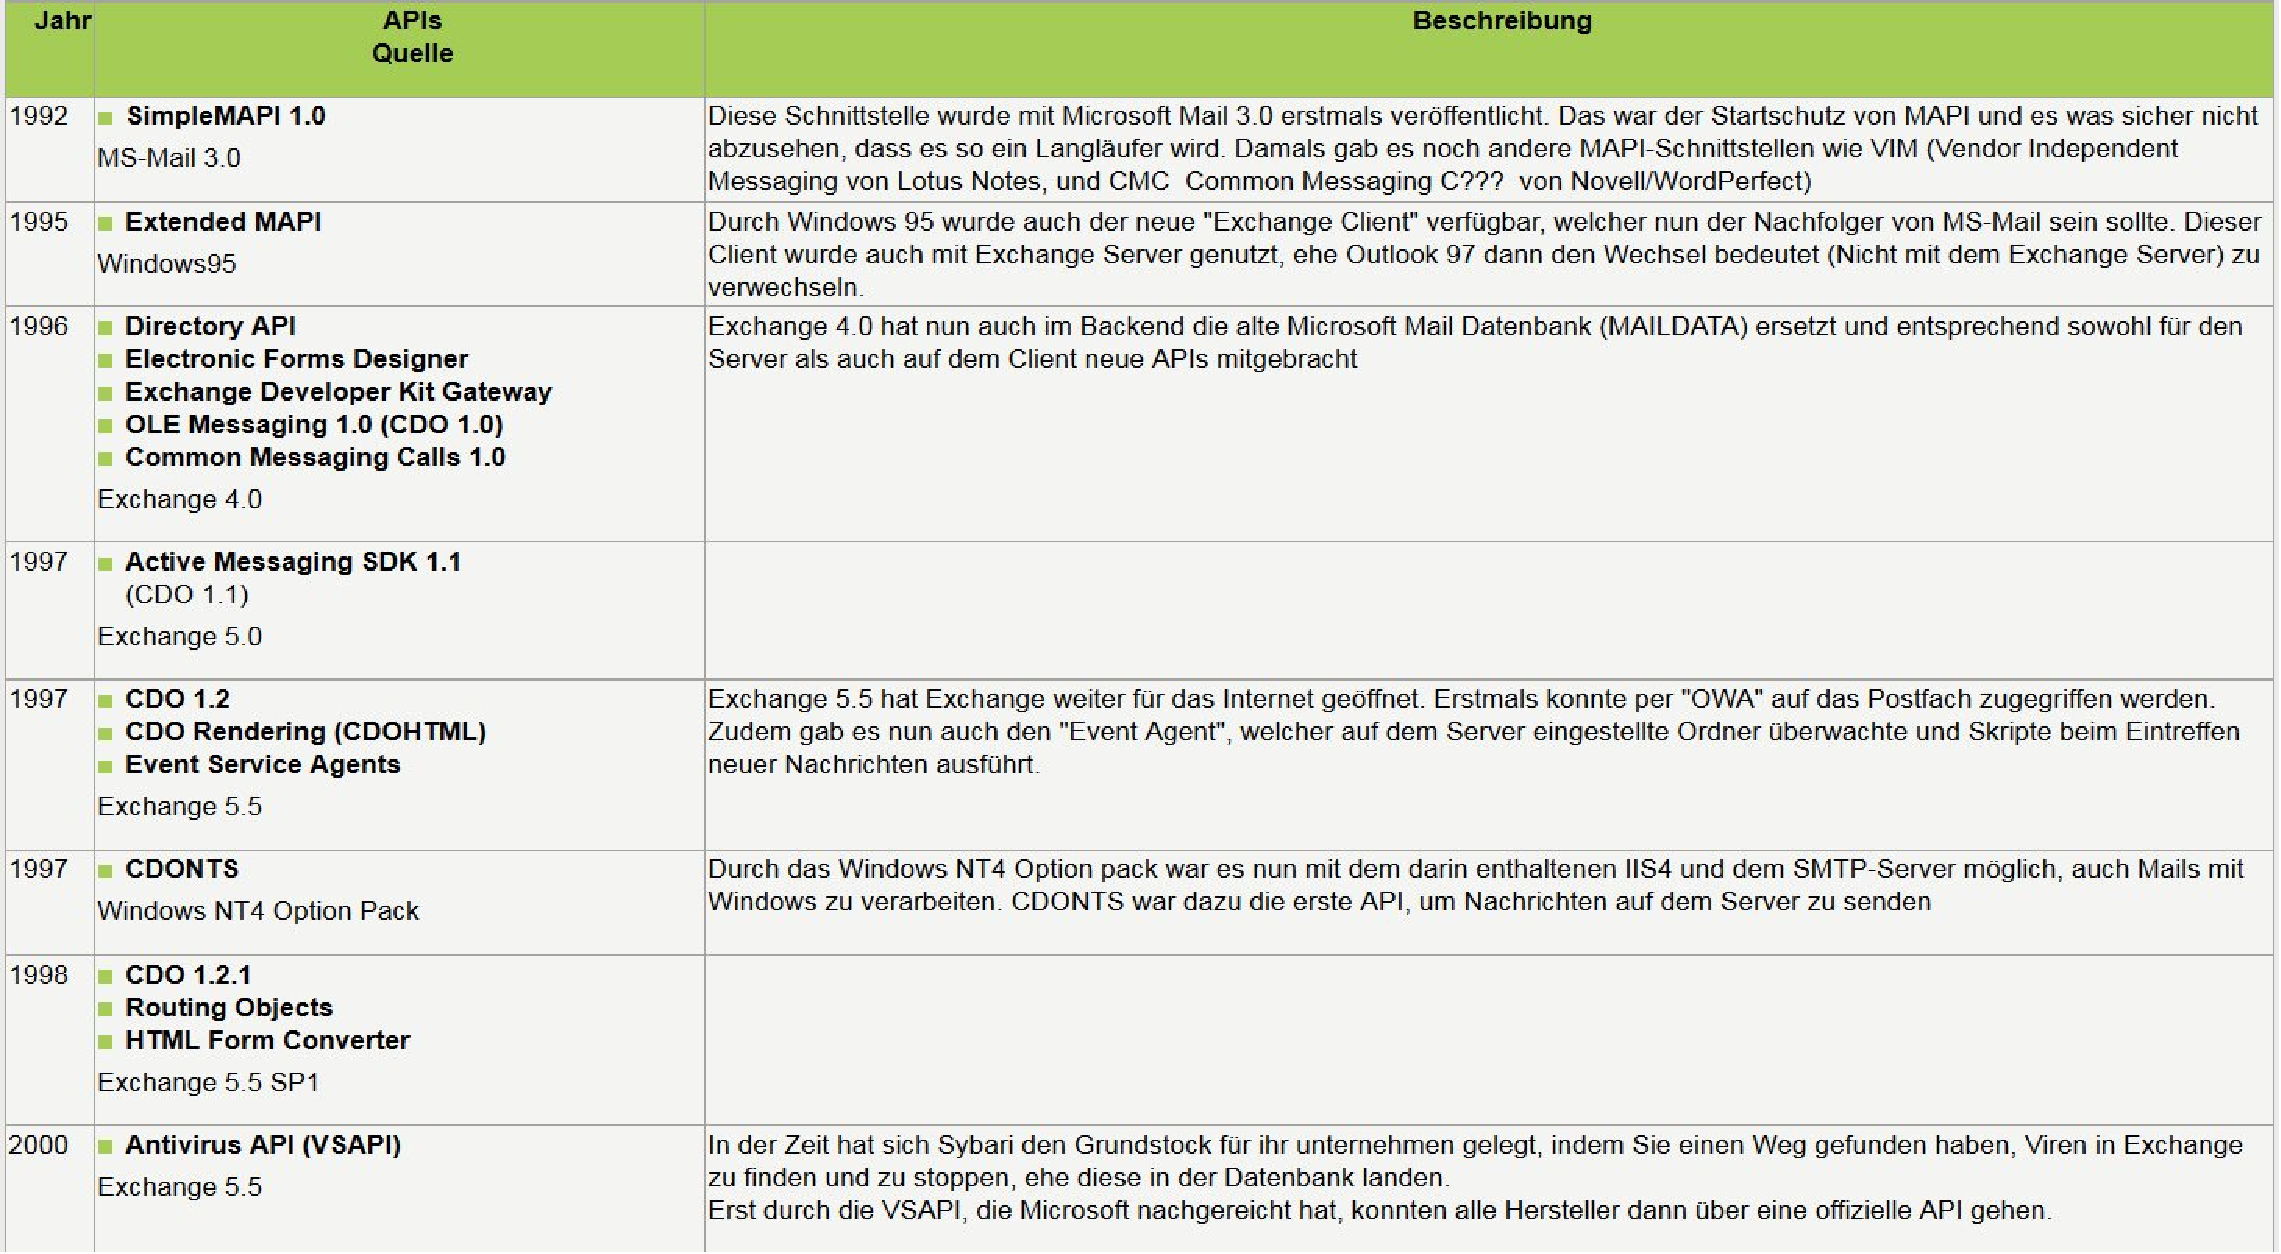
\includegraphics[width=1.0\textwidth]{Abbildungen/API_1.png}
\end{flushleft}
\label{API_1}
\begin{flushleft}
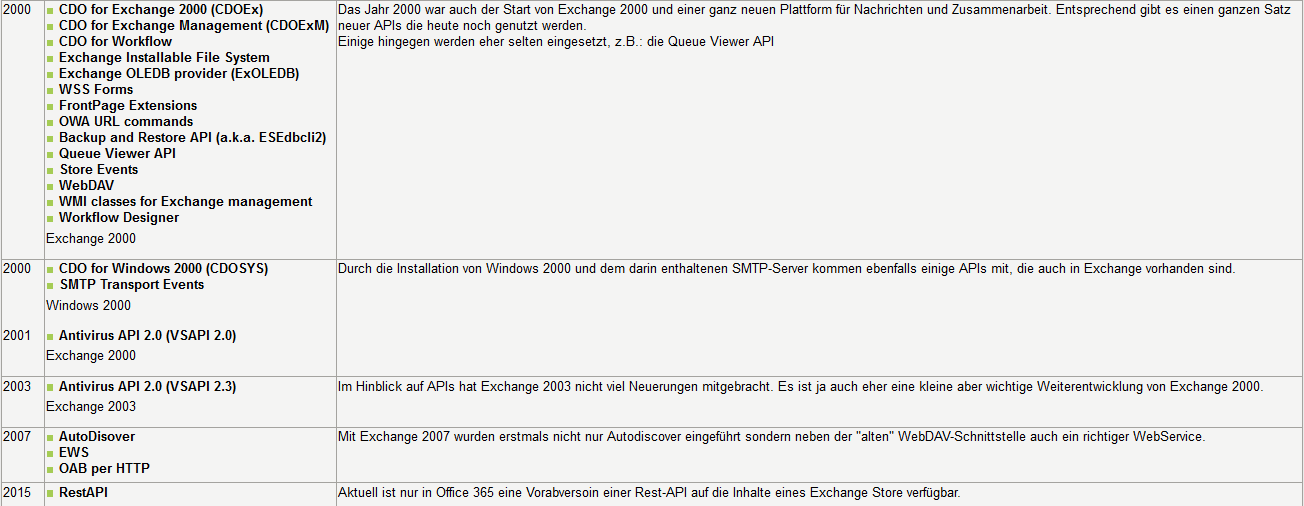
\includegraphics[width=1.0\textwidth]{Abbildungen/API_2.png}
\end{flushleft}
\noindent Quelle: http://www.msxfaq.de/code/wege.htm

\newpage

\begin{flushright}
Anhang 3\\
Blatt 3\\
\end{flushright}

\newpage

\begin{flushright}
Anhang 4\\
Blatt 6\\
\end{flushright}

\newpage

%-------------------------------------------------------------------------------------------------------
%					Literaturverzeichnis
%-------------------------------------------------------------------------------------------------------
\addsec{Literaturverzeichnis} %vergebe keine Kapitelnummer
\noindent
Widl, M (2015): Mircosoft Office 365. Das umfassende Handbuch, 3., aktualisierte Auflage, Bonn\\
\noindent
Joos, T. (2013): Microsoft Exchange Server 2013 - Das Handbuch, Köln

% Recherche Websiten für Service Desk
\noindent
http://venturebeat.com/2014/01/22/help-desk-software-heres-some-of-the-best-and-most-interesting/, 22. Mai 2014

\noindent
http://web.appstorm.net/roundups/communication-roundups/10-online-support-and-help-desk-apps/, 20. März 2015

\noindent
http://www.capterra.com/help-desk-software/ , Oktober 2015

\noindent
http://www.pcmag.com/article2/0,2817,2489457,00.asp , 22. März 2016

\end{document}
